\documentclass{article}

\usepackage{graphicx}
	\graphicspath{ {images/} }
\usepackage{wrapfig}
\usepackage{paralist}


\setlength{\parindent}{0pt}

\begin{document}

\begin{wrapfigure}{R}{0.40\textwidth}

\includegraphics[width=0.40\textwidth]{sarah.png}
\end{wrapfigure}
\textbf{\Large Sarah Garrell (20)} \\ \\
\textbf{Job Title: }1st year HR student\\
\textbf{Education:} High School + CEGEP\\
\textbf{Experience:}
\begin{compactitem}
\item Starbucks Barista
\item Summer camp counselor
\end{compactitem}
\textbf{Goals:}
\begin{compactitem}
\item Get her degree and work in recruiting
\item Pass accounting and finance
\end{compactitem}
\bigskip 
\textbf{Goals and Tasks user accomplishes}\\
Mostly she is worried about her finance class so anything that would help her with that would be appreciated.\\ \\
\textbf{Problem calculator solves} \\
She needs a calculator to calculate the equations for finance class. Her school does not allow her a programmable calculator so she will need to memorize the equations. She would definitely appreciate a it if she could enter the equation from left to right just like she memorized them.
\pagebreak

\subsection*{Interview Q\&A}
\textbf{What do you use a calculator for?}
\begin{itemize}
\itemsep0em 
\item Almost exclusively for her accounting and finance classes
\item Most of her usage of the calculator is for simple lightweight math used in accounting and finance.
\item She does not use it extensively, mostly for exams and homework.
\end{itemize}

\textbf{What would you like your calculator to do? Or what is the ideal calculator for you?}
\begin{itemize}
\itemsep0em 
\item She likes her calculator to be simple
\item Prefers a calculator that has its function symbols identical to the ones in the books
\item She would like her calculator to display the answers in a human readable form (5x7 Matrix numeric representation), and not the digital form (7-segment numeric representation)
\item In the future she would like to see a calculator network system, similar to that of the iclicker, where the professor would give you a password, which after inputting it into the calculator, downloads a custom function from the professor's base station, or unlocks/locks some of the pre programmed functions in the calculator.
\end{itemize}

\textbf{What kinds of calculators have you used? (physical, apps, online, etc.). Hardware or Software?}
\begin{itemize}
\itemsep0em 
\item Uses both a physical calculator as well as a calculator app on her phone.
\item Mainly uses the calculator application because it’s always available.
\item Prefers the physical calculator since she enjoys the tactile feel of the buttons and because phones are not allowed during exam time.
\end{itemize}

\textbf{What functions do you use most often? Which ones do you use the least?}
\begin{itemize}
\itemsep0em 
\item Most of the time she uses functions such as: addition, subtraction, delete (backspace) , $10^x$, Ans function for retrieving the previous answer , exponential and square root.
\item Rarely, if ever, uses logarithms or any of the trigonometric functions.
\end{itemize}

\textbf{What features did you like most about your calculator. What do you not like about your calculator?}
\begin{itemize}
\itemsep0em 
\item She feels indifferent about what she likes in her calculator. All she cares about is that the calculator gives the right answer.
\item The only thing she does not like about her calculator is that it displays numbers in a digital format (7 segment numeric representation)
\end{itemize}

\textbf{Are the aesthetics of your calculator important? What matters most (shape, color,  personalized themes, etc.)?}
\begin{itemize}
\itemsep0em 
\item Most of the physical aesthetics are of little importance to her. What matters the most is that the calculator gives an answer.
\item She claims that the physical aesthetics would be merely a perk and would not pay extra for them.
\end{itemize}

\textbf{If you’re using a keyboard, how would you map the keys to functions, numbers, etc. ergonomics?}
\begin{itemize}
\itemsep0em 
\item She would like her calculator to have some shortcuts to common functions such as percentage 
\item Prefers the shortcuts to have their own dedicated buttons on the calculator instead of having to press multiple buttons at once.
\end{itemize}

\textbf{Thoughts on making a calculator that has customizable capabilities? }
\begin{itemize}
\itemsep0em 
\item She would like to have the ability to program functions into the calculator, but only if academic establishments would allow it. 
\end{itemize}
\pagebreak

\begin{wrapfigure}{R}{0.4\textwidth}
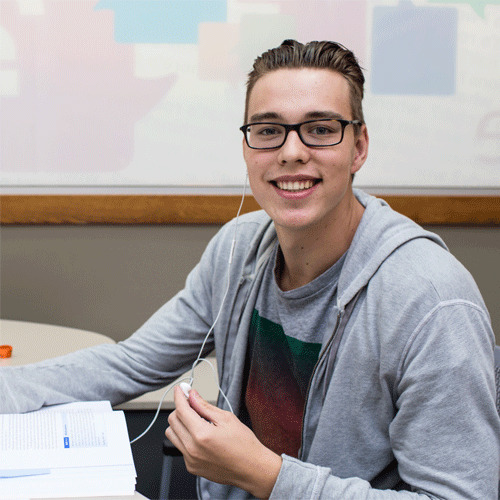
\includegraphics[width=0.4\textwidth]{kevin2.jpg}
\end{wrapfigure}
\textbf{\large Kevin Donnavan (23)} \\ \\
\textbf{Job Title: }Engineering Student\\
\textbf{Education:} 3rd Year Mechanical Engineering\\
\textbf{Experience:}
\begin{compactitem}
\item 3rd Year Mechanical Engineering
\item Summer internship as a junior structural engineer
\item Army reserves - Infantry
\end{compactitem}

\textbf{Skills:}
\begin{compactitem}
\item Problem Solving, Mathematics
\item Programming in Java, C\#, and C++
\end{compactitem}

\textbf{Goals:}
\begin{compactitem}
\item Obtain a good GPA and find a job in his field.
\end{compactitem}
\bigskip 
\textbf{Goals and Tasks user accomplishes}\\
Kevin says he just wants to get through his classes and get a decent GPA. Like everyone, his hardest classes mostly have to do with math (although he feels he is better than average). Kevin will be happy with anything that can make his math calculations easier.\\ \\
\textbf{Problem calculator solves} \\
The calculator helps Kevin get fast answers to difficult math problems he sees in class. Without a calculator, he is not sure how he would calculate the various functions that he sees on a daily basis. The calculator has to be precise enough so he can get the right answer to complex solutions of differential equations but he is not willing to wait - calculation must be near-instantaneous.
\pagebreak

\subsection*{Interview Q\&A}
\textbf{What do you use a calculator for?}
\begin{itemize}
\itemsep0em 
\item University studies
\item Mostly finds himself using it for mathematical purposes. 
\end{itemize}

\textbf{What would you like your calculator to do? Or what is the ideal calculator for you?}
\begin{itemize}
\itemsep0em 
\item His  ideal calculator would not be missing essential functions like plus, minus, multiplication, exponents, and the basics. Other common functions he mentioned from University, include logs, derivatives, e, integrals, roots, square roots, and more. He believes it’s a must to have the ANS (answer button), and calculation history included too. 
\item The calculator should be lightweight and portable. 
\item In the future he would like to see more calculators that provide more support for polar coordinates. Lastly he would like to have access to shorter readable manuals or video content to quickly go over all of the calculator’s features and how to implement them.
\item Believes It would be great to have the answer button, calculation history, polar capability and a shorter readable manual! 
\end{itemize}

\textbf{What kinds of calculators have you used? (physical, apps, online, etc.). Hardware or Software?}
\begin{itemize}
\itemsep0em 
\item Both softwares and physical.
\item Prefers physical calculator more than software-based because he has become used to it since his High School years. 
\item He doesn’t mind using software calculators as long as it has useful shortcuts. He defined a simple software calculator as something that can open and run quickly on a computer or any other device. 
\item Kevin also mentioned he uses software calculators mostly for basic problems but not derivations and more advanced operations because it becomes too tedious to work with. He would much rather use the physical one. 
\end{itemize}

\textbf{What functions do you use most often? Which ones do you use the least?}
\begin{itemize}
\itemsep0em 
\item Addition, subtraction, multiplication, division, exponents, roots, converting to fractions, sin, cos, tan, exponents, logs, and mod.
\end{itemize}

\textbf{What features did you like most about your calculator. What do you not like about your calculator?}
\begin{itemize}
\itemsep0em 
\item He liked Hexadecimal conversion, octa, binary conversions, derivations, and integration functions because they’re relevant to his engineering courses. .
\item Kevin doesn’t like using the mouse pointer on his computer to input the values and functions on his software-based calculator. He would much rather use the computer keyboard. He mentioned the clicking option should be removed completely to encourage others to use the keyboard. 
\end{itemize}

\textbf{Are the aesthetics of your calculator important? What matters most (shape, color,  personalized themes, etc.)?}
\begin{itemize}
\itemsep0em 
\item Easy to fit in your palm, portable, not too colourful (greyish, black). It should also be key mappable if it is a software-based calculator.
\end{itemize}

\textbf{If you’re using a keyboard, how would you map the keys to functions, numbers, etc. ergonomics?}
\begin{itemize}
\itemsep0em 
\item He would use the numbered keypad for inputting numbers 
\item Any symbols that are already commonly found (+,-,\^,etc.) on both computers and physical calculators should be included.
\item Assign important features and functions to large buttons, like the space bar or return key.
\item Include a shortcut to quit
\item Use the first letter of functions to input them into calculator. Ex: C for cos, S for sin, T for Tan, etc.
\end{itemize}

\textbf{Thoughts on making a calculator that has customizable capabilities? }
\begin{itemize}
\itemsep0em 
\item Doesn’t think it is necessary. He usually uses google to help solve complex problems and inputs the simple calculations on the calculator to double check his work and find the final answer. 
\item He believes it would be great to include physical skins to personalize the calculator but it is not a must.
\item In the future he would like to make it customizable by being able to download packages for calculator functions that can easily be added or removed to the device.
\end{itemize}
\pagebreak

\begin{wrapfigure}{R}{0.4\textwidth}
\includegraphics[width=0.4\textwidth]{tarek2.jpg}
\end{wrapfigure}
\textbf{\large Tarek Ghamzi (23)} \\ \\
\textbf{Job Title: }Engineering Student\\
\textbf{Job Title: }3rd year Electrical engineering student\\
\textbf{Education:} High School + CEGEP, currently in Electrical Engineering\\
\textbf{Experience:}
\begin{compactitem}
\item Subway
\item Pharmacist assistant
\end{compactitem}
\textbf{Skills:}
\begin{compactitem}
\item Problem Solving, Mathematics
\item Programming in C++ , and arduino 
\end{compactitem}
\textbf{Goals:}
\begin{compactitem}
\item Finish his degree with a good GPA
\item Find a job in his field
\end{compactitem}
\bigskip 
\textbf{Goals and Tasks user accomplishes}\\
Tarek claims that his main priority in life at the moment is to get his degree in Electrical Engineering. He claims that his field is heavily based on math, which he struggles with.
He aims to graduate with a higher than average GPA to gain an edge over others in his highly competitive field.\\ \\
\textbf{Problem calculator solves} \\
His calculator helps him in computing the high level mathematical functions that would take hours to solve by himself. It also helps him double check his answers for simple calculations.
Tarek claims that his calculator is with him at all times. Its accuracy, speed and comfort are of highest value to him.
\pagebreak

\subsection*{Interview Q\&A}
\textbf{What do you use a calculator for?}
\begin{itemize}
\itemsep0em 
\item Any mathematics courses in his degree
\item Almost all Engineering courses.
\item Counting money at his job 
\end{itemize}

\textbf{What would you like your calculator to do? Or what is the ideal calculator for you?}
\begin{itemize}
\itemsep0em 
\item It should have the basic, essential functions such as square root, exponential, logarithms, and trigonometric functions.
\item His ideal calculator would also have the ability to find variable unknowns (system of equations) 
\item He believes that a calculator that can plot and display graphs would be very beneficial
\item Another feature he would like to see in calculators is the ability to calculate indefinite integrals.
\item One of the main features he really wants to see is the ability to save/transfer his work (Graphs, functions, answers) from his calculator to his mobile phone.
\end{itemize}

\textbf{What kinds of calculators have you used? (physical, apps, online, etc.). Hardware or Software?}
\begin{itemize}
\itemsep0em 
\item He has used all kinds of calculators, physical ones, apps, software…
\item Prefers a physical calculator since he’s used to its layout and buttons
\item For quick calculations, he uses any calculator closest to him.
\end{itemize}

\textbf{What functions do you use most often? Which ones do you use the least?}
\begin{itemize}
\itemsep0em 
\item Frequently uses functions such as trigonometric functions, exponential, logarithms, and root
\item Hardly ever uses the modulus or absolute value functions.
\end{itemize}

\textbf{What features did you like most about your calculator. What do you not like about your calculator?}
\begin{itemize}
\itemsep0em 
\item He dislikes that his calculator does not support finding unknown variables in equations.
\item Claims that the few functions his calculator has for Radians and polar equations have been very helpful.
\end{itemize}

\textbf{Are the aesthetics of your calculator important? What matters most (shape, color,  personalized themes, etc.)?}
\begin{itemize}
\itemsep0em 
\item Aesthetics of his calculator are important to him.
\item He prefers his calculator to be comfortable to hold 
\item Personalized themes on his calculator have little importance to him
\item Prefers to buy a nice looking calculator that he likes and sticking with it instead of buying a customizable one.
\end{itemize}

\textbf{If you’re using a keyboard, how would you map the keys to functions, numbers, etc. ergonomics?}
\begin{itemize}
\itemsep0em 
\item He has no preference for key mapping, instead he would like his calculator to be set up in a way such that when he types the first few letters of the function name, it would show him function suggestions of which he can chose one.
\end{itemize}

\textbf{Thoughts on making a calculator that has customizable capabilities? }
\begin{itemize}
\itemsep0em 
\item Would only buy it if it comes at no extra cost, otherwise he would prefer to buy a cheaper calculator with the pre-programmed functions that he knows he needs.
\end{itemize}
\pagebreak






\begin{wrapfigure}{R}{0.40\textwidth}

\includegraphics[width=0.40\textwidth]{arash.jpg}
\end{wrapfigure}
\textbf{\Large Arash Mohajer (28)} \\ \\
\textbf{Job Title: }2nd year Avionics Engineering student \\
\textbf{Education:} High School + CEGEP, currently in University\\
\textbf{Experience:}
\begin{compactitem}
\item Completed two internships at a company that manufactures Flight Simulators
\item Worked part time as a waiter
\end{compactitem}
\textbf{Skills:}
\begin{compactitem}
\item Mathematics, Physics
\item Technical Writing
\item Some experience programming in C\# and Java
\end{compactitem}
\textbf{Goals:}
\begin{compactitem}
\item Find more internships during his degree
\item Finish his degree in a reasonable amount of time
\item Save money for his future (manage personal finance)
\end{compactitem}
\bigskip
\textbf{Goals and Tasks user accomplishes}\\
Arash wants to finish his degree in Avionics as soon as possible so that he can get a good job in a field that he enjoys. He wants to continue taking part in engineering competitions and hackathons to learn more about his field and others and to meet other like-minded individuals. He wants to manage his personal finance in order to pay off the debt that he currently has from his university tuition. \\ \\
\textbf{Problem calculator solves}
While he is more focused on graduating than getting good grades in his classes, he has many math and physics intensive classes where he relies on a calculator. He uses a calculator at school for homework, projects and exams. He also uses a calculator for conversion between different units for engineering and physics problems. At home, he uses his calculator to manage his personal finances and to plan his future spending. 
\pagebreak


\begin{wrapfigure}{R}{0.40\textwidth}
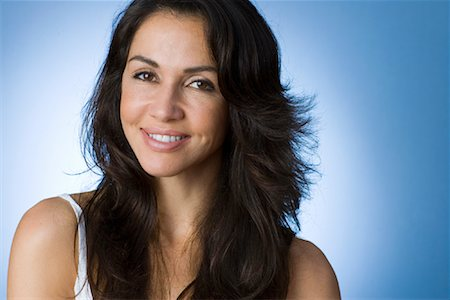
\includegraphics[width=0.40\textwidth]{victoria.jpg}
\end{wrapfigure}
\textbf{\Large Victoria Benlolo (35)} \\ \\
\textbf{Job Title: }1st year HR student\\
\textbf{Education:} High School + CEGEP, currently in University\\
\textbf{Experience:}
\begin{compactitem}
\item Completed two internships at a company that manufactures Flight Simulators
\item Worked part time as a waiter
\end{compactitem}
\textbf{Skills:}
\begin{compactitem}
\item Mathematics, Physics
\item Technical Writing
\item Some experience programming in C\# and Java
\end{compactitem}
\textbf{Goals:}
\begin{compactitem}
\item Find more internships during his degree
\item Finish his degree in a reasonable amount of time
\item Save money for his future (manage personal finance)
\end{compactitem}
\bigskip 
\textbf{Goals and Tasks user accomplishes}\\
Arash wants to finish his degree in Avionics as soon as possible so that he can get a good job in a field that he enjoys. He wants to continue taking part in engineering competitions and hackathons to learn more about his field and others and to meet other like-minded individuals. He wants to manage his personal finance in order to pay off the debt that he currently has from his university tuition. \\ \\
\textbf{Problem calculator solves}
While he is more focused on graduating than getting good grades in his classes, he has many math and physics intensive classes where he relies on a calculator. He uses a calculator at school for homework, projects and exams. He also uses a calculator for conversion between different units for engineering and physics problems. At home, he uses his calculator to manage his personal finances and to plan his future spending. 
\pagebreak










\subsection*{Interview Q\&A}
\textbf{What do you use a calculator for?}
\begin{itemize}
\itemsep0em 
\item He uses it to solve his math and physics problems most of the times. 
\item He also uses it to keep track of his finances and plan his spending accordingly.
\end{itemize}

\textbf{What would you like your calculator to do? Or what is the ideal calculator for you?}
\begin{itemize}
\itemsep0em 
\item In addition to basic functions he would like it to be able to calculate more complex functions such as $e^x$, log, roots, derivatives, integrals and so on.
\item His ideal calculator is the one that has specific button for each function while it is portable. 
\item Maybe a folding calculator.
\end{itemize}

\textbf{What kinds of calculators have you used? (physical, apps, online, etc.). Hardware or Software?}
\begin{itemize}
\itemsep0em 
\item He has used both hardware and software. 
\item He prefers using his engineering calculator app on his cellphone but since he is not allowed to use it in the exams he has to use his regular calculator most of the times.
\end{itemize}

\textbf{What functions do you use most often? Which ones do you use the least?}
\begin{itemize}
\itemsep0em 
\item These days in addition to basic functions like multiplication and division, he mostly uses functions such as power, exp, root, log, trigonometric, derivative and integral. 
\item The factorial function might be one of those that he used the least recently.
\end{itemize}

\textbf{What features did you like most about your calculator. What do you not like about your calculator?}
\begin{itemize}
\itemsep0em 
\item Since it is a pretty simple calculator, it is simple to use for the fundamental functions. 
\item The things that he doesn't like about it is that it cannot convert decimals into fraction and also it can`t calculate derivative and integral.
\end{itemize}

\textbf{Are the aesthetics of your calculator important? What matters most (shape, color,  personalized themes, etc.)?}
\begin{itemize}
\itemsep0em 
\item He doesn't care about the aesthetic of calculator.
\item Its simplicity of use, accuracy and portability have higher importance to him.
\end{itemize}

\textbf{If you’re using a keyboard, how would you map the keys to functions, numbers, etc. ergonomics?}
\begin{itemize}
\itemsep0em 
\item He would assign each function to a specific button. 
\item For inverse functions such as arcsin or nth root he would assign shift + the key for original function. 
\item He would make sure that his calculator has the ability to represent numbers in different formats. For instance, he would assign the key “H” for Hexadecimal and “R” for radian.  
\end{itemize}
\pagebreak

\begin{wrapfigure}{R}{0.40\textwidth}
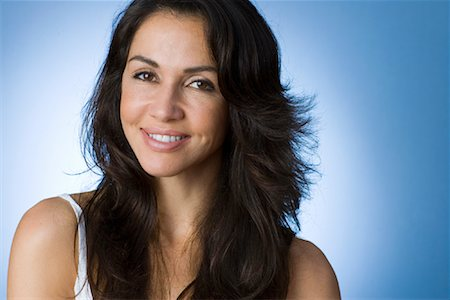
\includegraphics[width=0.40\textwidth]{victoria.jpg}
\end{wrapfigure}
\textbf{\Large Victoria Benlolo (35)} \\ \\
\textbf{Job Title: }1st year HR student\\
\textbf{Education:} High School + CEGEP\\
\textbf{Experience:}
\begin{compactitem}
\item Has owned and managed a spa for 2 years
\item Worked as a financial analyst for 7 years
\end{compactitem}
\textbf{Skills:}
\begin{compactitem}
\itemsep0em 
\item Economics, Business, Finance
\item Public Speaking
\item Investing
\end{compactitem}
\textbf{Goals:}
\begin{compactitem}
\itemsep0em 
\item Maximize the profit of her business
\item Invest in new profitable endeavours 
\item She is interested in opening new spas around town once her business grows more
\item Hire new employees and continue to manage the finances of her business
\end{compactitem}
\bigskip 
\textbf{Goals and Tasks user accomplishes}\\
Victoria wants to continue to grow her business and potentially start franchising her spa to open up new locations around the city. She wants to hire new talent in order to expand her finance team. Her day-to-day includes managing employees' pay, keeping inventory of products, paying bills and managing business income. Additionally, she wants to continue investing in the stock market. \\ \\
\textbf{Problem calculator solves}
At the Spa, Victoria uses a calculator to calculate all of her business expenses, profit/loss, employee salaries, etc. A reliable calculator is very important to her. She uses a calculator to plan expenses in her future business expansion plans.  She also uses a calculator to keep track of how her personal accounts and investment portfolios are growing. 
\pagebreak

\subsection*{Interview Q\&A}
\textbf{What do you use a calculator for?}
\begin{itemize}
\itemsep0em 
\item She mostly uses it to calculate the price of services and products for the clients. 
\item Calculate her employees’ salary based on the hours they work.
\item She also uses it to keep track of her personal finances.
\end{itemize}

\textbf{What would you like your calculator to do? Or what is the ideal calculator for you?}
\begin{itemize}
\itemsep0em 
\item Since most of the times she uses it to calculate the amount of money, she prefers her calculator to round the amount to 2 decimals.
\item She would also like to have a button to calculate the tax so it would save her time and prevent making mistakes.
\end{itemize}

\textbf{What kinds of calculators have you used? (physical, apps, online, etc.). Hardware or Software?}
\begin{itemize}
\itemsep0em 
\item She generally uses a physical calculator because she is used to it.
\item When she does not have her calculator with her, she uses apps and/or online calculators.
\end{itemize}

\textbf{What functions do you use most often? Which ones do you use the least?}
\begin{itemize}
\itemsep0em 
\item Most often she uses multiplication, addition, subtraction, division and percentage. 
\item She rarely uses other functions such as sin, cos or log.
\end{itemize}

\textbf{What features did you like most about your calculator. What do you not like about your calculator?}
\begin{itemize}
\itemsep0em 
\item She likes that its screen is large in size and that it has soft buttons.
\item Its simplicity to work with. 
\item Since it is rather large, it is not very portable. She can only use it in her work place.
\end{itemize}

\textbf{Are the aesthetics of your calculator important? What matters most (shape, color,  personalized themes, etc.)?}
\begin{itemize}
\itemsep0em 
\item Not that much. As long as it has a decent look and is easy to work with, it would be OK.
\end{itemize}

\textbf{If you’re using a keyboard, how would you map the keys to functions, numbers, etc. ergonomics?}
\begin{itemize}
\itemsep0em 
\item She would map the numbers and basic functions to their associated keys in keyboard.
\item She would also like to have some shortcut keys for instance “t” for calculating tax and “s” for total sum.
\item She believes it would be interesting to have a calculator that can be customized by the user. For example since the tax rates, products price and employees' salaries are subject to change, it would be cool if it had a shortcut for each of them to be able to modify the amount when the change happens. 
\end{itemize}
\pagebreak

\end{document}